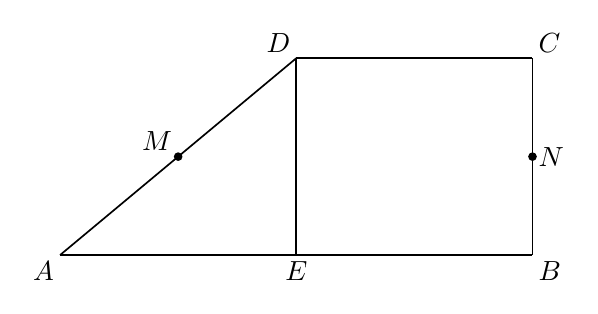
\begin{tikzpicture}[x=1cm,y=1cm,font=\normalsize,
 geometry edge/.style={solid,line width=.6pt},
 geometry mark/.style={solid,line width=.6pt},
 geometry label/.style={font=\normalsize,inner sep=2pt}]
\coordinate (A) at (-1,0);
\coordinate (E) at (2,0);
\coordinate (B) at (5,0);
\coordinate (D) at (2,2.5);
\coordinate (C) at (5,2.5);
\coordinate (M) at (0.5,1.25);
\coordinate (N) at (5,1.25);
\draw[geometry edge] (A)--(E);
\draw[geometry edge] (E)--(B);
\draw[geometry edge] (E)--(D);
\draw[geometry edge] (D)--(C);
\draw[geometry edge] (C)--(B);
\draw[geometry edge] (A)--(D);
\fill[black] (M) circle[radius=0.055];
\fill[black] (N) circle[radius=0.055];
\node[geometry label,below left] at (A) {$A$};
\node[geometry label,below] at (E) {$E$};
\node[geometry label,below right] at (B) {$B$};
\node[geometry label,above left] at (D) {$D$};
\node[geometry label,above right] at (C) {$C$};
\node[geometry label,above left] at (M) {$M$};
\node[geometry label,right] at (N) {$N$};
\end{tikzpicture}
